\renewcommand{\thesection}{S7}
\section{Simulation Results and Validation}

\subsection{Static Simulations}
    For both static simulations in which the structure was subjected to launch-phase conditions with 8g of acceleration, a mesh convergence study was conducted. Figure \ref{fig:MeshConvergence} presents a graph of the maximum von Mises stress (MPa) versus the number of mesh elements, showing that the results stabilize with mesh refinement. This confirms the validity of the obtained stress values. The blue curve corresponds to the I-beam profile, and the orange curve to the manufacturable version.

    \renewcommand{\thefigure}{S24}
    \begin{figure}[ht]
        \centering
        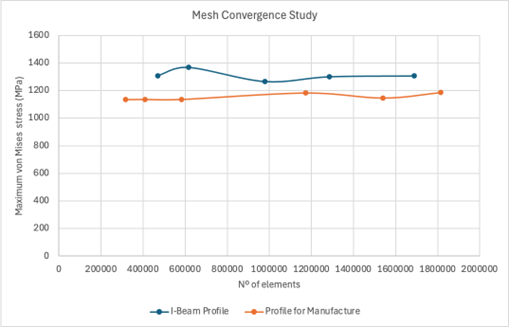
\includegraphics[height=6cm]{Figures/MeshConvergence.png}
        \caption{Maximum von Mises stress vs. number of elements for static simulations under launch-phase loading (8g), showing convergence for the I-beam (blue) and manufacturable profile (orange).}
        \label{fig:MeshConvergence} 
    \end{figure}
    \vspace{-20pt} % Adjust this value to reduce the space
    \FloatBarrier

    For the same simulation, Figure \ref{fig:Displacement} shows the maximum displacement (URES, total resultant displacement, in millimetres), with the I-beam on the left and the manufacturable configuration on the right. The results indicate peak values of 17 mm and 32 mm, respectively. It is also worth noting that the maximum displacement values consistently converged with mesh refinement, as previously discussed.

    \renewcommand{\thefigure}{S25}
    \begin{figure}[ht]
        \centering
        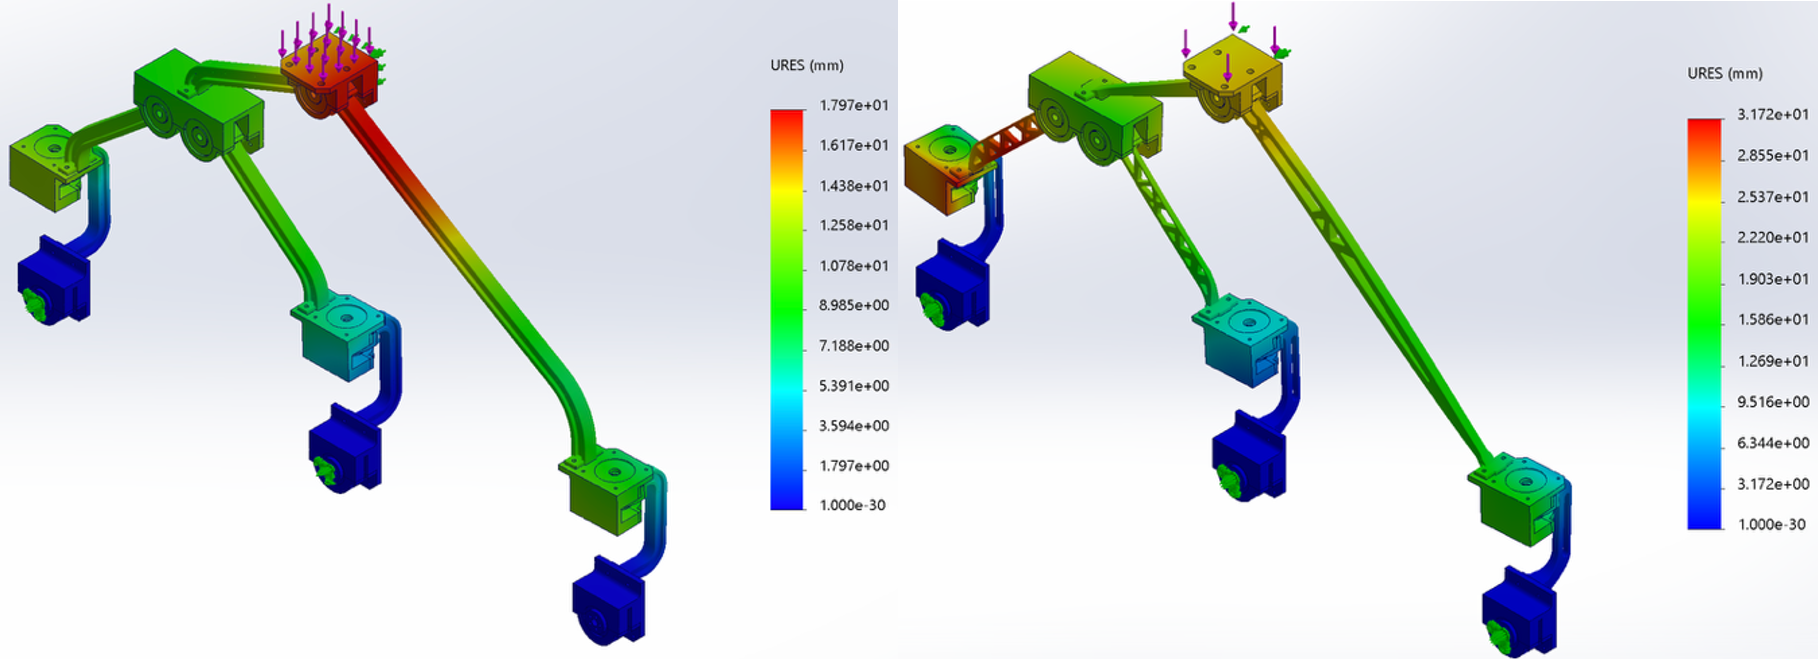
\includegraphics[height=5.5cm]{Figures/Displacement.png}
        \caption{Maximum displacement (URES) from static simulations under launch-phase loading (8g). Comparison between the I-beam (left) and manufacturable configuration (right).}
        \label{fig:Displacement} 
    \end{figure}
    \vspace{-20pt} % Adjust this value to reduce the space
    \FloatBarrier